% LTex: language=pl
\section{Architektura wdrożenia}
\subsection{Topologia logiczna}
Wraz ze zmianą technologii, na której oparta była architektura wdrożenia systemu STOS, zmianie musiała ulec również architektura rozwiązania.

\begin{figure}[!h]
	\begin{center}
		\resizebox{0.7\textwidth}{!} {
			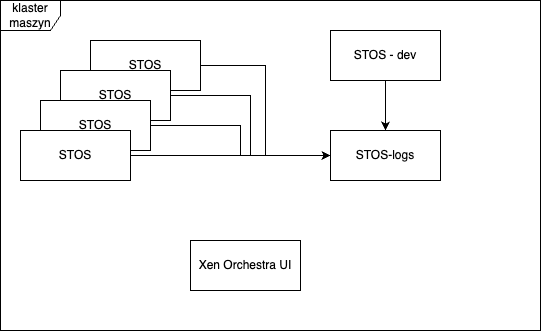
\includegraphics{img/4/wdrozenie.png}
		}
		\caption[Topologia wdrożenia systemu STOS]{Diagram przedstawiający topologię wdrożenia platformy serwerowej systemu STOS opartego na wirtualizacji oferowanej przez xcp-ng. Źródło własne.}
		\label{diagramTopologiaStos}
	\end{center}
\end{figure}

\noindent Diagram \ref{diagramTopologiaStos} przedstawia klaster i komponenty wdrożonego systemu STOS jako maszyny wirtualne. W ramach rozpatrywania komponentów samego systemu należy zwrócić uwagę na trzy główne rodzaje maszyn: \textit{STOS}, \textit{STOS-dev} i \textit{STOS-logs}. W porównaniu z proponowanym rozwiązaniem opartym o zastosowanie klastra Kubernetes można zaobserwować diametralnie zmniejszoną liczbę osobnych bytów z perspektywy architektury wdrożenia. Z racji o wiele większych kosztów związanych z wdrożeniem i uruchomieniem maszyny wirtualnej w porównaniu z kontenerem, logiczne grupowanie serwisów i ich enkapsulacja odbywa się na poziomie całej maszyny wirtualnej, co pozwala na logiczne rozdzielenie części systemu odpowiedzialnych za podobne funkcjonalności, jak i uproszczenie protokołu komunikacji między serwisami, które ściśle ze sobą współpracują. Na szczególną uwagę zasługuje zmiana w architekturze głównych komponentów platformy serwerowej systemu STOS -- serwisu zarządzającego \textit{"manager"} i modułu kompilującego \textit{"worker"}. Dzięki wdrożeniu ich na jednej maszynie wirtualnej zniknęła konieczność korzystania z protokołu http w ramach komunikacji pomiędzy tymi dwoma serwisami, dzięki czemu złożoność programów uległa zmniejszeniu. Podobna zmiana dotyczy funkcjonalności agregacji logów z systemu STOS, ponieważ wszystkie serwisy odpowiedzialne za procesowanie logów zostały umieszczone w ramach jednej maszyny wirtualnej.
\noindent Wadą enkapsulacji zrealizowanej w ten sposób, w porównaniu z rozwiązaniem o większej granularności wykorzystywanym przez systemy korzystające z orkiestratorów kontenerów, jest potencjalnie mniejsza niezawodność takiego systemu. Takie powiązanie ze sobą komponentów systemu może prowadzić do mniejszej dostępności usług w przypadku wystąpienia awarii, co w systemach klasy przemysłowej jest jednym z krytycznych czynników stanowiących o jakości dostarczanego systemu. Jednakże, w kontekście systemu STOS, o stosunkowo niskim stopniu złożoności w kontekście architektonicznym, wystąpienie takich sytuacji jest stosunkowo mało prawdopodobne, a czasy naprawy awarii systemu są dosyć niskie z uwagi na rozmiar wdrażanej platformy.

\subsubsection{STOS}
Jest to główna maszyna wirtualna, niezbędna do funkcjonowania systemu STOS. Jest to również jedyna maszyna, która może być skutecznie replikowana i skalowana horyzontalnie. Na każdą maszynę STOS przypada jedna instancja serwisu zarządzającego \textit{"manager"} i jedna lub więcej instancji modułu kompilującego \textit{"worker"}, współpracujących z lokalnym serwisem zarządzającym. Maszyna ta komunikuje się z istniejącym serwerem webowym systemu STOS w celu pobierania zadań studentów do ewaluacji i maszyną \textit{STOS-logs} przesyłając logi działania aplikacji.

\subsubsection{STOS-dev}
Maszyna wirtualna, stanowiąca wierną kopię maszyny produkcyjnej \textit{STOS} pod względem środowiska. Służy ona testowaniu wprowadzanych przez zespół deweloperski zmian w środowisku produkcyjnym bez wdrażania tych zmian w środowisku, w którym miałyby one wpływ na działanie systemu doświadczane przez użytkowników systemu. Podobnie jak w przypadku maszyny \textit{STOS}, przesyła ona logi działania aplikacji w ramach komunikacji z maszyną \textit{STOS-logs}, lecz nie korzysta ona z istniejącego, zewnętrznego systemu pobierania zadań do ewaluacji, zamiast tego wykorzystując lokalnie działającą symulację takiego serwera.

\subsubsection{STOS-logs}
Jest to maszyna wirtualna odpowiedzialna za wszystkie funkcjonalności systemu związane z gromadzeniem, wyszukiwaniem i wizualizacją logów aplikacji. Uruchomione są na niej serwisy Logstash, Elasticsearch i Kibana, pozwalające na odbieranie logów otrzymywanych przez maszyny systemu STOS, wydajne ich indeksowanie i wizualizację w formie tablic \textit{(dashboardów)}. \textit{STOS-logs} komunikuje się zarówno z maszynami \textit{STOS}, jak i maszynami odgrywającymi rolę środowiska deweloperskiego \textit{STOS-dev}. 

\subsection{Aspekty sieciowe}
W porównaniu do rozwiązania opartego o klaster Kubernetes, konfiguracja komunikacji między serwisami w ramach sieci przy wdrażaniu systemu opartego o nadzorcę \textit{(hypervisor)} xcp-ng jest bardziej złożona. Topologia systemu w kontekście sieci została przedstawiona na diagramie \ref{diagramSiecStos}.
\begin{figure}[!h]
	\begin{center}
		\resizebox{0.7\textwidth}{!} {
			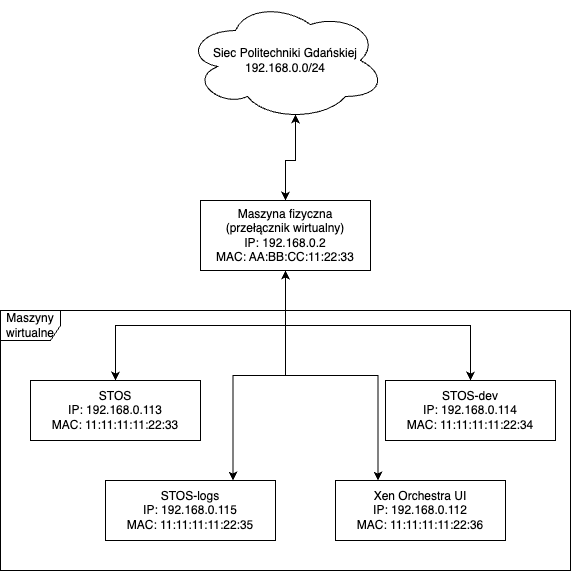
\includegraphics{img/4/wdrozeniesiec.png}
		}
		\caption[Topologia sieciowa wdrożonego systemu STOS]{Diagram przedstawiający topologię systemu STOS w kontekście sieci. Adresy IP i MAC są wyłącznie przykładowymi adresami. Źródło własne.}
		\label{diagramSiecStos}
	\end{center}
\end{figure}
\noindent Centralnym komponentem topologii sieciowej systemu jest maszyna fizyczna, na której zainstalowany jest program nadzorcy \textit{(hypervisor)}. Xcp-ng korzysta z oprogramowania Open vSwitch uruchomionego w ramach maszyny fizycznej, w celu umożliwienia konfiguracji sieciowej maszyn wirtualnych w taki sposób, aby znajdowały się one w tej samej podsieci, co maszyna fizyczna \cite{xcpNetwork}. Realizowane jest to za pomocą wirtualnego przełącznika sieciowego warstwy drugiej, co pozwala na wydajną obsługę ruchu sieciowego, zarówno między maszynami będącymi częściami systemu, jak i między maszynami wirtualnymi a systemami zewnętrznymi \cite{vswitch}.
\noindent Kolejnym elementem konfiguracji sieciowej wdrożenia jest interakcja z siecią Politechniki Gdańskiej, w której znajduje się system. Z racji braku możliwości dostępu do konfiguracji podsieci, w której znajdują się maszyny fizyczne i utrudnionej komunikacji z administratorami sieci politechnicznej, należało dostosować się do istniejących ograniczeń nałożonych na urządzenia znajdujące się w sieci. Najbardziej restrykcyjnym z nich była polityka dotycząca przyznawania statycznych adresów IP, które są ściśle powiązane z adresem MAC urządzenia. Dodatkowo ruch wychodzący z urządzenia o adresie IP nieodpowiadającemu adresowi MAC przypisanemu do niego na poziomie zarządzania siecią jest filtrowany, co efektywnie uniemożliwia wykorzystanie adresów IP niezatwierdzonych przez administratorów sieci. Warto odnotować, że o ile uniemożliwia to komunikację zewnętrzną, o tyle maszyny wirtualne w ramach systemu STOS są nadal w stanie komunikować się ze sobą nawet w przypadku braku skonfigurowanego odgórnie adresu IP. Efektywnie, taka sytuacja prowadzi do konieczności pozyskania od administratorów sieci Politechniki Gdańskiej nowej pary adresów IP-MAC za każdym razem, gdy należy wdrożyć nową maszynę wirtualną mającą komunikować się z systemami i urządzeniami spoza wdrożonego klastra xcp-ng.
\subsection{Administracja}
Wbudowane w program nadzorcy xcp-ng rozwiązanie pozwalające na administrację klastrem wirtualnym oparte jest o wiersz polecenia i szereg poleceń, które mogą zostać uruchomione z poziomu terminala maszyny fizycznej, jak i za pomocą zdalnego ich wywołania za pomocą protokołu ssh. Zaletą takiego podejścia jest możliwość bardziej precyzyjnej konfiguracji systemu i szybka diagnostyka ewentualnych awarii. Jednakże wymaga ono znajomości dość ekstensywnej listy komend, co prowadzi do istnienia dość wysokiego progu wejścia dla potencjalnego administratora systemu. 
\noindent Rozwiązaniem wykorzystanym przy wdrożeniu platformy serwerowej dla systemu STOS jest \textit{Xen Orchestra}. Jest to aplikacja dedykowana do administracji klastrami maszyn opartych na xcp-ng rozwijana przez firmę Vates, która jest również autorem xcp-ng. Xen Orchestra uruchomiona jest w formie osobnej maszyny wirtualnej mieszczącej się na klastrze i pozwala na wykonywanie wszystkich najważniejszych z perspektywy administratora systemu operacji, takich jak zarządzanie maszynami wirtualnymi, zdalny dostęp do maszyn i zarządzanie wewnętrzną siecią klastra za pomocą graficznego interfejsu użytkownika w formie strony internetowej \cite{xoa}. Skorzystanie z tego rozwiązania pozwala na stosunkowo szybkie i proste wdrożenie administratorów systemu STOS i udostępnienie im podstawowych funkcjonalności pozwalających na monitorowanie i zarządzanie klastrem, jednocześnie zachowując funkcjonalności zarządzania za pomocą wiersza poleceń, przeznaczoną dla bardziej zaawansowanych użytkowników.
